\documentclass[12pt]{article}

\usepackage{graphicx}
\usepackage{paralist}
\usepackage{listings}
\usepackage{booktabs}

\oddsidemargin 0mm
\evensidemargin 0mm
\textwidth 160mm
\textheight 200mm

\pagestyle {plain}
\pagenumbering{arabic}

\newcounter{stepnum}

\title{Assignment 1 Solution}
\author{Donisius Wigie - wigied}
\date{\today}

\begin {document}

\maketitle

The modules ReadAllocationData.py and CalcModule.py are used to allocate first year engineering students into their second year programs. ReadAllocationData.py will read relevant data from files and put them into a form specified by the assignment. CalcModule.py performs operations on the data and allocates the first year students into their second year programs.

\section{Testing of the Original Program}

My approach towards coming up with the testing module was to think of ways in order to automate the module as much as possible. I wanted the test cases to make as little assumptions as possible about the code. This involves not having to change the format of the files, and providing input by creating data by itself.

I created a function to test the sort function and see if it actually sorted the gpas of the students in descending order. 

I also created a function failures(s) to obtain a list of macIDs who have a gpa that is less than 4.0 using the list of dictionaries produced by readStdnts.

The belongOrNot(A, F) function is to determine if any of the students who have a gpa below 4.0 were allocated into a second year program. It takes the list of students who failed produced by  failures(s) and the dictionary of allocations produced by allocate(S, F, C). 

The firstChoices(F, S) function puts the macIDs of the first choice students along with their first choice into a list so it is convenient for the fcAllocated(A, fc) function to see if everyone who had first choice got their first choice pick.

These functions are used to test all regular inputs. The first four test cases were just regular input tests to see if the CalcModule functions will work for inputs which should be obvious.

For boundary cases, I tried to think of as many as I could which are possible inputs a user could provide the programs. The first boundary case is to see if the function can handle an empty department capacity file. The first boundary case forced me to think of a way to deal with an empty department list. In the beginning of my allocate function I added a feature which makes sure the department capacity file is not empty or missing any of the seven streams. It also tests to see if it could deal with an empty student file. Another boundary case regarding department list tests to see if allocate can deal with greater number of students who have a gpa of 4.0 or over than there are department seats. I needed to let the user know that there is not enough space or not all students are able to be allocated. I added a feature in my allocate function that checks to see that there is enough department space for the students.

The third boundary case is to test the average function by entering a non-male or non-female gender as the gender input. Ideally the function would raise an exception. 

The fourth boundary case is to test if allocate can handle students with a negative gpa. This was not an issue in my program as it checks if the gpa is below 4.0 before allocating.The fifth boundary case which tests if allocate can handle students with a gpa above 12 properly raised issues for me. I fixed this by checking to see if gpa is below or equal to 12 in addition to checking if gpa is above or equal to 4.0 before allocating.

The sixth boundary case is to see if the average function can handle an empty list. This raised a problem in my average function since it would cause my program to try to divide by 0. I fixed this by checking to see if the list is empty and terminating before being able to carry out the rest of the operations.

I also added tests to see if allocate can handle nonsensical inputs which I dealt with by adding a feature to see if the S-input is of type list, if the F-input is of type list and if the C-input is of type dictionary.

My allocate function has a feature which deals with the unlikely chance that an overwhelming amount of people choose the same three top choices and some do not get allocated into any department. In that case, my allocate function will let the user know that 'macID' has not been allocated into any function and they will be put into a random department temporarily until the issue is resolved. I could not think of a way to automate this testing since people may deal with this is a multitude of ways, so I will test the one case manually and see if the program deals with it in a fair way.


\section{Results of Testing Partner's Code}

The outputs for my test driver used on my partners code:

\medskip

\begin{center}
	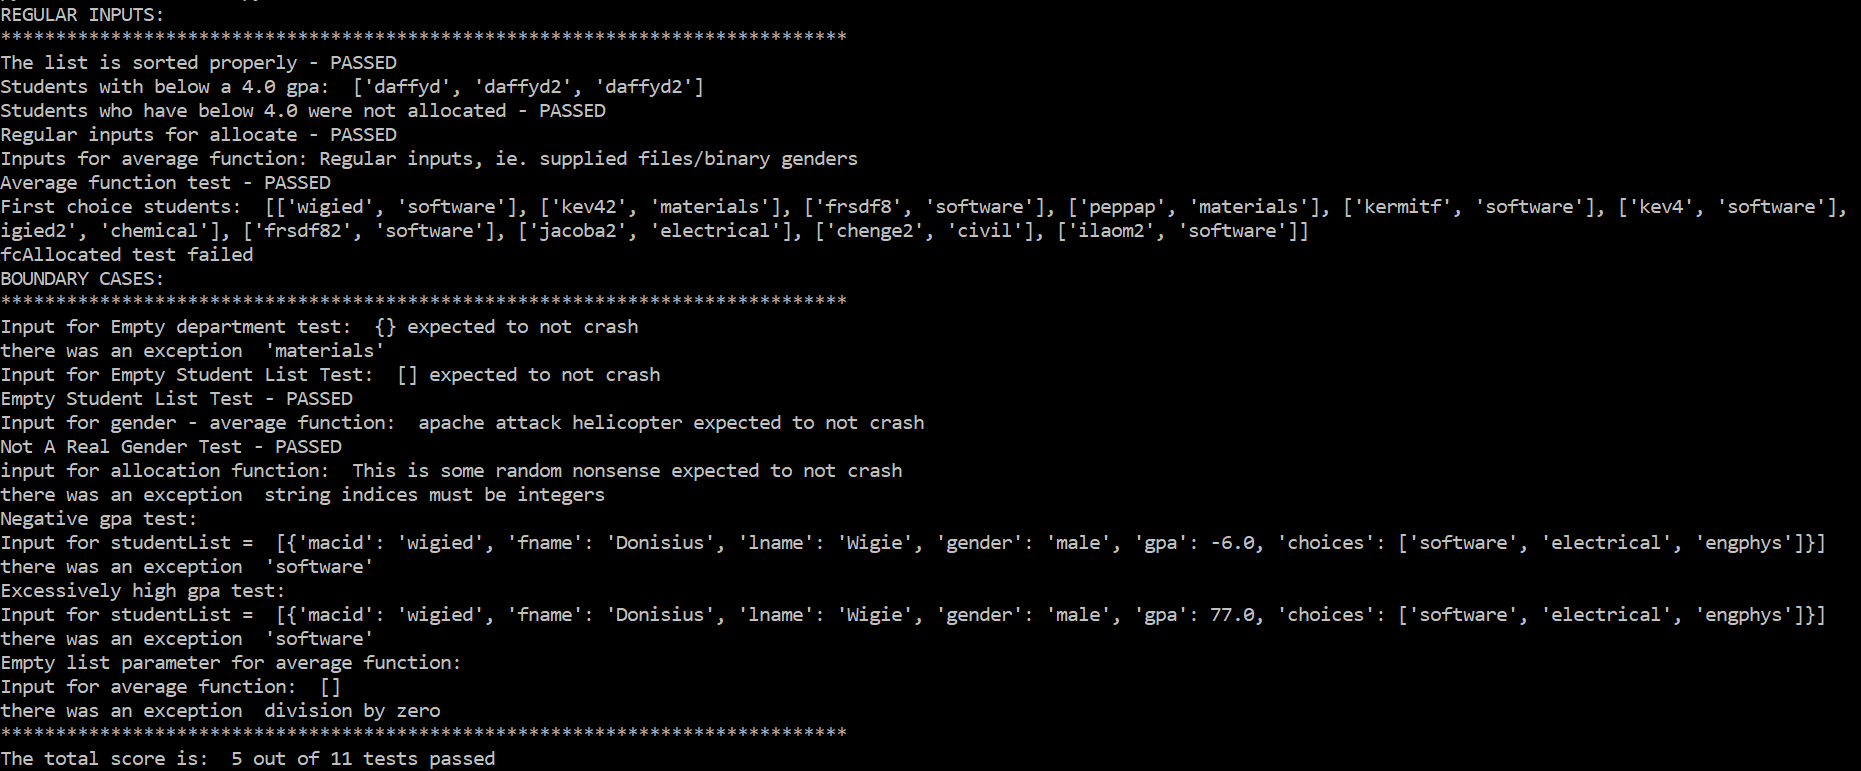
\includegraphics{a1}
\end{center}

After putting my partner's code through my test driver, it passed 5 out of 11 of the tests. The code was able to pass the regular inputs except for the allocation of all free choice students. 
My partner's code was able to pass 2/7 of the boundary case tests. It passed the empty student list test for the allocate function and the not a real gender input for the average function.
For the allocate function, the code failed the empty department test, the random nonsense inputs test, the negative gpa test and the excessively high gpa test.
For the average function, it failed the empty list test.

\section{Discussion of Test Results}
While creating the testCalc.py module, it brought up a lot of issues with my code that I would not have thought about if I was not actively looking for ways my program could be broken. I mentioned earlier that I went into the creation of my test module with the idea of trying to make a little assumptions possible. After putting my partner's code through my test driver, the test results made me realize that some of my test cases make too many assumptions. The best example is the "nonsense" inputs where the test driver would generate an input for the functions which do not have the right input type. The reason I do not think this is a good test is because when someone abuses the program like that by providing input which makes no sense, you can sometimes argue that it may be better just to allow the program to crash. I made the assumption that the program should catch the exception and that is why the test gives me points for that. Someone else could assume that it should just allow it to crash and that is why the test does not give them points. As mentioned earlier, in the event that an overwhelming majority of people choose the same three top choices and some students are unable to be allocated into any of their top choices, then it would just place them into temporary spots. I needed to do this test manually, but looking at my partner's code they also made this same assumption.  

\subsection{Problems with Original Code}

In my discussion of the test results, I commented that in the process of creating my testCalc.py module, it brought up a lot of issues with my code. The most obvious issue was the empty student list for the average function. I did not consider an empty student list as a possible output and because of this I did not realize that an empty list would cause a division by zero to occur. From this I created multiple test cases for my allocate function to deal with empty input and the empty dictionary (empty department) caused issues. I fixed this by checking if it is empty and if there is enough total seats across all departments for all the students. I also did not consider how my program would deal with a gpa greater than 12.0, which I fixed by not allocating anyone who has a gpa less than 4.0 or greater than 12.0.

\subsection{Problems with Partner's Code}

My test driver brought up some problems with my partner's code, many of which my code had before I came up with the test cases. The first test that failed showed that not everyone who had free choice did not get their first choice department. My functions to test this determined someone did not get allocated and when I manually checked some free choice students did not get put into their first choice. The second test that failed showed that the allocate function is not able to deal with an empty department list or when there are more students with a passing gpa than there are seats for them to be allocated into. The third test that failed showed that it isn't able to catch the nonsense input exceptions which as mentioned in my discussion of the test results is not entirely wrong. The fourth and fifth tests that failed showed that the program is not able to deal with incorrect grade inputs, i.e, negative gpa or a gpa above 12.0. The sixth test that failed showed that the average function is not able to take an empty list otherwise a division by zero would occur.


\section{Critique of Design Specification}
The specification of this assignment imposed design decisions which in my opinion could be improved upon. For example, a better implementation for storing the information of the students would be to store the information in a student class for each student. It would be a lot easier to change and access information regarding each student if all the information is stored in a student class. I think keeping the names of students with free choice in a list was a simple but effective design specification since it is easy to access. Another way is to also keep this information in the student class mentioned earlier. This might make it slightly harder to quickly access all free choice names, and slightly easier to know if each individual student has free choice. I believe keeping the information in a list was still a good design decision. As for department capacities I can not think of a better way of implementing that. 
%\newpage

\section{Answers to Questions}

\begin{enumerate}[(a)]

\item average(L, g) can be made more general by being able to get the average of more than exclusively male or exclusively female. For example a more flexible average function would also be able to take another input (eg. 'all') and take the average of all the students present in the student list input. Another feature that would make the average function more flexible can be to calculate the anticipated cut off average for the departments based off the grades of the students, the demand for each department, and the actual amount of space available in each department. Such a feature would be a difficult task to implement but would make the function extremely versatile. Along a similar line of thinking, sort(s) could be made more general by being able to sort in both ascending order or descending order depending on what the user wants.

\item We were allowed to make the assumption that aliasing will not occur in the dictionaries in our lists which in this context means that making changes in one dictionary will affect the others. In general, aliasing is a concern with dictionaries because dictionaries in python are mutable. If you create a variable to take the value of a dictionary and change the variable in any way, the original dictionary will also change. A way that you may guard against this is to create a new instance of the same dictionary instead of making them all connected to the same original dictionary. I implemented such a feature in my readStsnts function.

\begin{center}
	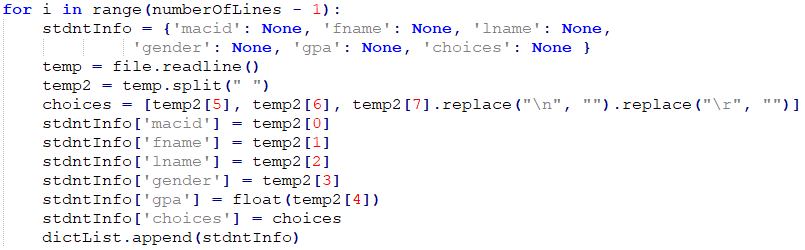
\includegraphics{a12}
\end{center}

In readStdnts, I instantiate a different dictionary by putting a new dictionary inside the for loop. This is done in order to create a different dictionary for each student and to avoid the problems that dictionaries have with aliasing.

\item The ReadAllocationData.py module is very difficult to test since the way the data is stored in the files is open-ended and because of this it could vary greatly in how people implement this module. For example, you may implement the data files as a csv and use functions to parse the csv files. Or you can just have a regular text file and have the data be organized in any way you want. Because it is so open ended, it is hard to come up with test cases for ReadAllocationData.py and that is why CalcModule.py was selected as the one to be tested. Some test cases to test ReadAllocationData.py can be to see if the functions put the data into the correct form, i.e, does the readStdnts function create a list of dictionaries containing the students' macIDs, lastnames, firstnames, gpas, and program choices? Is the free choice in list form? Is the department capacities in a dictionary? 

\item One problem of using strings as keys in several dictionaries and to represent members of finite sets is that it can be prone to typos. It is very convenient to use strings as representations of members of finite sets. For dictionaries in particular , it could cause many strange issues. Since there is very little protection against misspelled field names and field names can be removed or added easily at any time in a dictionary, it can cause the program to add or remove fields unintentionally. A better approach would be to use namedtuple. By using a namedtuple, it solves this issue by ensuring that the correct field names are used. In addition, namedtuples are also more memory efficient than regular classes.

\item The mathematical notion of a tuple is a finite ordered sequence of elements. Other options for implementing this in python is by writing a custom class. Classes allow you to define data structures which may be reused and provide the same set of fields with every instantiation. Similar to a structure in C, a python custom class may be created in order to mimic a data structure which stores various information. The way that the information would be stored is by providing the data through a tuple and creating a new instance of the class. I would definitely recommend changing the data structure used in the code modules to use this custom class, as it is much neater and less error prone. I would create the custom student class as follows:

\begin{center}
	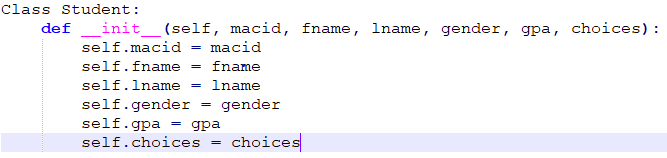
\includegraphics{a13}
\end{center}

\item If the list of strings was changed to a different data structure like a tuple, then the CalcModule.py wouldn't need to be modified since although a tuple can not be modified, the information is still able to be accessed. In CalcModule.py, there is no need to modify the list of strings for the student's choices, only access to the information is needed. If a custom class was written for students and CalcModule was modified accordingly, then CalcModule would still need to be modified further. The way that my program goes through the student information and checks the choices to allocate the students accordingly is to parse through the information using a for loop. It loops through the top 3 choices and checks if there is room in the first choice department and if not move on to the second choice and if not then move on to the third choice. In order to use the methods from the custom class, I would need to change the implementation to index the choices of the students using the function and not a loop, and to check for true if there is no other choices. This implementation is a lot more flexible as it is able to adapt to an increase in the number of top choices a student can have. Students can also have a different number of top choices.

\end{enumerate}

\newpage

\lstset{language=Python, basicstyle=\tiny, breaklines=true, showspaces=false,
  showstringspaces=false, breakatwhitespace=true}
%\lstset{language=C,linewidth=.94\textwidth,xleftmargin=1.1cm}

\def\thesection{\Alph{section}}

\section{Code for ReadAllocationData.py}

\noindent \lstinputlisting{../src/ReadAllocationData.py}

\newpage

\section{Code for CalcModule.py}

\noindent \lstinputlisting{../src/CalcModule.py}

\newpage

\section{Code for testCalc.py}

\noindent \lstinputlisting{../src/testCalc.py}

\newpage

\section{Code for Partner's CalcModule.py}

\noindent \lstinputlisting{../partner/CalcModule.py}

\newpage

\section{Makefile}
\lstset{language=make}

\noindent \lstinputlisting{../Makefile.}

\end {document}